\documentclass{beamer}
\usepackage[utf8]{inputenc}
\usepackage[slovak]{babel}
\usepackage{caption}

\usetheme{CambridgeUS}
\setbeamercolor{title}{bg=red!65!black,fg=white}
\setbeamercolor{item}{fg=red}
\captionsetup[figure]{labelfont={color=red}, name=Obrázok}
\usenavigationsymbolstemplate{}


\begin{document}
	
\title[Detekcia a oprava kolísavých bitov v~RF]{Detekcia a oprava kolísavých bitov v~sade registrov}
\author{Dávid Bolvanský}
\institute[FIT VUT]{Systémy odolné proti poruchám}
\date{}

	
\frame[plain]{\titlepage}

\begin{frame}\frametitle{Kolísavé (erratic) bity}
\begin{itemize}
	\item \textit{erratic} \-- kolísavý, nepredvídateľný, nevyspytateľný
	\item častý dôvod jednobitových chýb počas fáze zápisu/mazania buniek
	\item chyby spôsobené výkyvmi \footnote{trapping/detrapping of electrons and holes in the gate oxide} vo $V_{min}$ (minimálna hodnota napätia, pri ktorej je zaručená správna činnosť)
	\item erratic bit vykazuje nestále a nepredvídateľné správanie pri mazaní \-- jeho hraničná hodnota napätia sa náhodne mení v~každom cykle
	\item ide o~druh občasných chýb, kde sa bity a ich hodnoty javia ako uviaznuté (stuck) 
	\item poškodená bunka nemusí byť schopná zmeniť hodnotu pri zápise $\rightarrow$ čítanie nesprávnych hodnôt
	\item jav prvotne pozorovovaný na Flash pamätiach, neskôr aj na SRAM (registre)
\end{itemize}
\end{frame}

\begin{frame}\frametitle{Ochrana sady registrov (Register File, RF)}
\begin{itemize}
	\item prístup do registrov je veľmi častý $\rightarrow$ ochrana je nevyhnutná pre zabránenie šíreniu ďalších chýb do častí systému, inak hrozí pád programov alebo poškodenie dát
	\item TMR, ECC sa nepoužívajú (vysoká cena vo forme plochy na čipe, oneskorenia) $\rightarrow$ použitie parity, ktorá umožňuje detekciu jednobitovej chyby
	\item ak je chyby detegovaná, opravenie (opätovné spustenie inštrukcie) je možné len v~prípade, keď inštrukcia, ktorá spôsobila chybnú hodnotu, neopustila zreťazenú linku (pipeline) 
	\item registre s~poškodenými bitmi je vo všeobecnosti nutné natrvalo zakázať $\rightarrow$ zníženie počtu dostupných registrov, čo vedie k~nižšiemu výkonu, prípadne až k~celkovej nefunkčnosti
	\item vzniká potreba hľadania nových techník na riešenie chýb spôsobenými trvalými chybnými bitmi za cenu mierne zvýšenej réžie
\end{itemize}
\end{frame}

\begin{frame}\frametitle{Metóda na zvýšenie odolnosti RF voči kolísavými bitmi}
\begin{itemize}
	\item jedná sa jednoduchý a efektívny mechanizmus
	\item oprava chýb spôsobenej kolísavými bitmi sa vykonáva priamo v~sade registrov
	\item mechanizmus pri detekcii chyby zisťuje, či sa jedná o~problém kolísavých bitov alebo o~soft chybu
	\item identifikuje kolísavý bit a opraví chybu bez nutnosti ďalších informácií
	\item metóda využíva fakt, že občasné chyby kvôli kolísavým bitmi spôsobia, že niektoré bity budú uviaznuté na hodnote $0$ alebo $1$ po nejakú dobu
	\item nezáleží teda na tom, akú hodnotu do bitu zapíšeme, vždy sa prečíta rovnaká hodnota
\end{itemize}
\end{frame}

\begin{frame}\frametitle{Princíp metódy}
\begin{center}
\begin{figure}
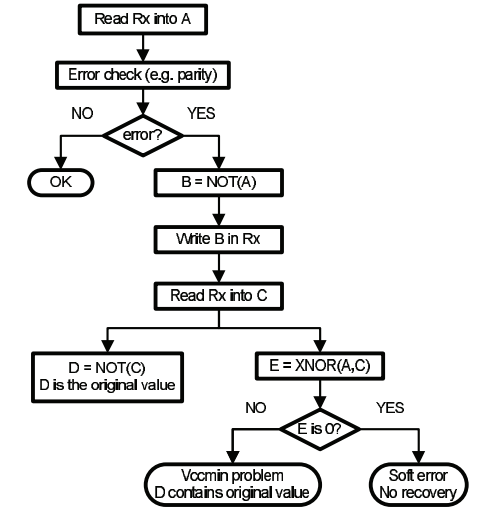
\includegraphics[width=\textwidth,height=0.7\textheight,keepaspectratio]{method.png}
\caption{Detekcia a oprava chyby spôsobenej kolísavými bitmi}
\end{figure}
\end{center}
\end{frame}

\begin{frame}\frametitle{Popis metódy}
\begin{enumerate}
	\item prečítame hodnotu z~registra $Rx$ $\rightarrow$ hodnota $A$
	\item oprava chyby začína, keď kontrola parity hodnoty $A$ zistí chybu
	\item je nutné zistiť, či chyba bola spôsobená kolísavým bitom, a opraviť ju 	(proces opravy je jednoduchý vďaka vlastnosti uviaznutia hodnoty u~kolísavých bitov)
	\item invertujeme prečítanú hodnotu $A$ $\rightarrow$ hodnota $B$
	\item zapíšeme hodnotu $B$ späť do registra $Rx$
	\item znova prečítame register $Rx$, získanú hodnotu $C$  z~registra $Rx$ invertujeme $\rightarrow$ hodnota $D$
	\item vypočítame $E= XNOR(A,C)$
	\item ak $E = 0$ \-- jedná sa o~soft chybu
	\item ak $E \neq 0$ \--  ide o~prípad kolísavého bitu $\rightarrow$ hodnota $D$ sa zhoduje s~pôvodnou a správnou hodnotu
	\item chyba bola úspešne opravená
\end{enumerate}
\end{frame}

\begin{frame}\frametitle{Príklad činnosti metódy}
\begin{center}
	\begin{figure}
		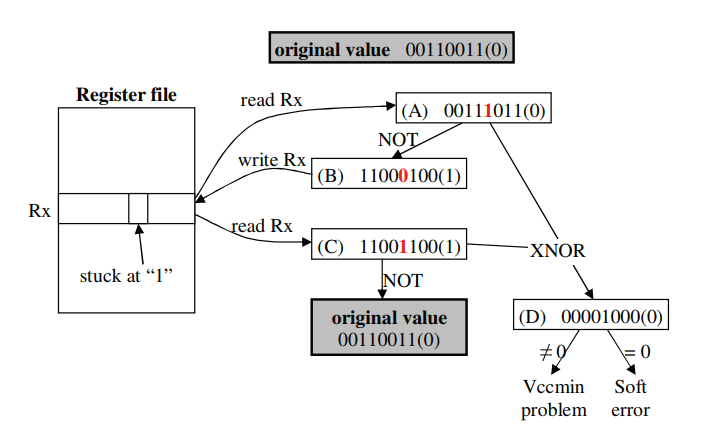
\includegraphics[width=\textwidth,height=0.7\textheight,keepaspectratio]{example.png}
		\caption{Detekcia a oprava chyby spôsobenej kolísavými bitmi}
	\end{figure}
\end{center}
\end{frame}

\begin{frame}\frametitle{Réžia metódy}
\begin{itemize}
	\item cena je z~pohľadu výkonu a HW veľmi nízka
	\item pri detekcii chyby (ktorej výskyt nie je častý) sa procesor pozastaví (stall) a vykoná sa pár jednoduchých operácií (invertovanie, XNOR)
	\item pridaná réžia teda spočíva v~pár krokoch potrebných na obnovu hodnoty a jej zápis
\end{itemize}
\end{frame}

\begin{frame}\frametitle{Alternatívne prístupy}
\begin{itemize}
	\item replikácia hodnôt registrov do nepoužívaných registrov pre obnovu z~prechodných a soft chýb \-- ak ECC zistí chybu, správna hodnota je získaná z~nepoškodeného registra, ktorý obsahuje replikovanú hodnotu
	\item replikácia častí procesoru \-- napr. IBM G5 replikuje frontend procesoru a všetky inštrukcie vykonáva paralelne dvakrát $\rightarrow$ porovnaním výstupu inštrukcií zisťuje chyby  $\rightarrow$ pre obnovu z~chýb si udržuje kópiu sady registrov
\end{itemize}
\end{frame}

\begin{frame}\frametitle{Zdroje}
Primárny zdroj
\begin{itemize}
	\item Online Error Detection and Correction of Erratic
	Bits in Register Files
	\url{https://ieeexplore.ieee.org/document/5195987}
\end{itemize}
Sekundárne zdroje
\begin{itemize}
	\item Erratic Fluctuations of SRAM Cache Vmin at the 90nm Process Technology Node
	\url{https://ieeexplore.ieee.org/document/1609436}
	
	\item Erratic Bit Errors in Latches
	\url{https://ieeexplore.ieee.org/document/4227672}
	
	\item Analysis of erratic bits in flash memories
	\url{https://ieeexplore.ieee.org/document/995831}
	
	\item Error Correction Codes for Non-Volatile Memories
	\url{https://www.springer.com/la/book/9781402083907}
\end{itemize}
\end{frame}

\end{document}